\begin{figure}
\centering
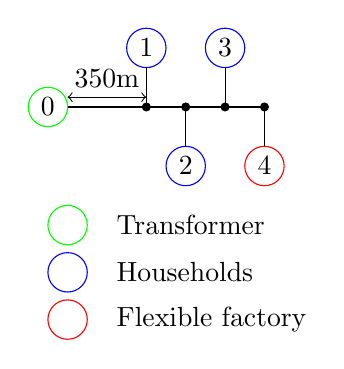
\begin{tikzpicture}[scale=0.5]
\draw (0,0) -- (5,0);
\draw [color=green] (-0.5,0) circle (0.5cm);
\node at (-0.5,0) {0};
\draw (2,0) -- (2,1);
\draw [fill=black] (2,0) circle (0.1cm);
\draw [color=blue] (2,1.5) circle (0.5cm);
\node at (2,1.5) {1};
\draw (3,0) -- (3,-1);
\draw [fill=black] (3,0) circle (0.1cm);
\draw [color=blue] (3,-1.5) circle (0.5cm);
\node at (3,-1.5) {2};
\draw (4,0) -- (4,1);
\draw [fill=black] (4,0) circle (0.1cm);
\draw [color=blue] (4,1.5) circle (0.5cm);
\node at (4,1.5) {3};
\draw (5,0) -- (5,-1);
\draw [fill=black] (5,0) circle (0.1cm);
\draw [color=red] (5,-1.5) circle (0.5cm);
\node at (5,-1.5) {4};
\draw [<->] (0, 0.25) -- (2, 0.25);
\node [above] at (1,0.25) {350m};
\draw [color=green] (0,-3) circle (0.5cm);
\node [right, xshift=0.5cm] at (0,-3) {Transformer};
\draw [color=blue] (0,-4.2) circle (0.5cm);
\node [right, xshift=0.5cm] at (0,-4.2) {Households};
\draw [color=red] (0,-5.4) circle (0.5cm);
\node [right, xshift=0.5cm] at (0,-5.4) {Flexible factory};
 \end{tikzpicture}
\caption{The real distribution network used.}
\label{fig:schema_line}
\end{figure}
